\documentclass[10pt,letterpaper]{article}
\usepackage[top=0.85in,footskip=0.75in,marginparwidth=2in]{geometry}

\usepackage{graphicx}% http://ctan.org/pkg/graphicx
\usepackage{amsmath,amsfonts} % Math packages
\usepackage{amsthm}
\usepackage{mathtools}
\usepackage{caption}
\usepackage{subcaption}
\usepackage{bbm}
\usepackage{bm}
\usepackage{listings}

% Definitions of handy macros can go here
\newcommand{\ths}{\textsuperscript{th}{\,}}
\DeclareRobustCommand{\stirling}{\genfrac\{\}{0pt}{}}
\newcommand\Multi{\ensuremath{\mathrm{Multi}}}
\newcommand\Uniform{\ensuremath{\mathrm{Uni}}}
\newcommand\Beta{\ensuremath{\mathrm{Beta}}}
\newcommand\Bernoulli{\ensuremath{\mathrm{Bern}}}
\newcommand\Dirichlet{\ensuremath{\mathrm{Dir}}}
\newcommand\GammaDist{\ensuremath{\mathrm{Gamma}}}
\newcommand\CRP{\ensuremath{\mathrm{CRP}}}
\newcommand\GEM{\ensuremath{\mathrm{GEM}}}
\newcommand\N{\ensuremath{\mathcal{N}}}
\DeclareMathOperator{\E}{\mathbb{E}}
\newcommand{\indpath}[2]{\mathbin{\mathcal{P}{\left(#1,#2\right)}}} % induced path
\newcommand\indic[1]{\ensuremath{\mathbbm{1}\left(#1\right)}}
\newcommand{\SPT}{\mathcal{T}}
\newcommand{\GSPT}{\overline{\SPT}}
\newcommand{\SPN}{\mathcal{S}}
\newcommand{\X}{\mathbf{X}}
\newcommand{\C}{\mathbf{C}}
\newcommand{\loss}{\mathcal{L}}
\newcommand{\K}{\mathbf{K}}
\newcommand{\kk}{\mathbf{k}}
\newcommand{\data}{\mathcal{D}}
\newcommand{\x}{\mathbf{x}}
\newcommand{\y}{\mathbf{y}}
\newcommand{\xn}{\mathbf{x}_{n}}
\newcommand{\new}{_{*}}
\newcommand{\xnd}{x_{n,d}}
\newcommand{\xd}{\mathbf{x}_{\cdot,d}}
\newcommand{\z}{\mathbf{z}}
\newcommand{\ks}{\mathbf{k}}
\newcommand{\ProductNode}{\mathsf{P}}
\newcommand{\SumNode}{\mathsf{S}}
\newcommand{\SumNodes}{\bm{\mathsf{S}}}
\newcommand{\Leaf}{\mathsf{L}}
\newcommand{\Child}{\mathsf{C}}
\newcommand{\Root}{\ensuremath{\mathbf{root}}}
\newcommand{\ch}{\ensuremath{\mathbf{ch}}}
\newcommand{\scope}{\ensuremath{\mathbf{sc}}} % leaf function
\newcommand{\leafs}[1]{\mathbin{\mathbf{leafs}(#1)}} % leaf function
\newcommand{\w}{w}
\newcommand{\cond}[2]{\mathbin{\left. #1\nonscript\;\middle|\nonscript\; #2 \right.}}

\newtheoremstyle{mystyle}{}{}{}{}{\bf}{}{\newline}{}
\theoremstyle{mystyle}
\newtheorem*{definition}{Definition}
\newtheorem{theorem}{Theorem}

% bibtex
\usepackage[
backend=biber,
style=alphabetic,
sorting=ynt
]{biblatex}
\addbibresource{references.bib}

\begin{document}
\title{Combining Gaussian Processes with Sum-Product Networks}
\author{}

% make the title area
\maketitle
\section{Introduction}
This write-up gives a brief overview on some possibilities to combine Gaussian processes with sum-product networks.
At first I will give a short recap on SPNs as well as on GPs and introduce the necessary notations. Throughout this work I generally refer to generalized sum-product networks \cite{Peharz2015} as sum-product networks only, i.e. SPNs with leaves representing arbitrary distributions.

\subsection{Sum-Product Network}
\label{sec:spns}
A sum-product network (SPN) \cite{Poon2011} over random variables $X_1, \dots, X_D$ is a rooted directed acyclic graph whose leaves are univariate or multivariate distributions and whose internal nodes are sums and products. 
For ease of use, we will use $\Leaf$ to denote a leaf node, $\SumNode$ to denote a sum node, $\ProductNode$ to denote a product node, $\Child$ to denote a child node of a sum or product, and $\SPN$ to denote the SPN.
Each edge $(\SumNode,\Child)$ emanating from a sum node $\SumNode$ has a non-negative weight $\w_{\SumNode,\Child}$ and the value of a sum node is $\SumNode(\x) = \sum_{\Child \in \ch(\SumNode)} \w_{\SumNode,\Child} \Child(\x)$, where $\ch(\SumNode)$ are the children of $\SumNode$ and $\Child(\x)$ is the value of node $\Child$. For simplicity, we assume that $\sum_{\Child \in \ch(\SumNode)} \w_{\SumNode,\Child} = 1$. The value of a product node is the product of the values of its children and the value of a leaf node is computed according to the probability density function of the distribution associated with the node. 
The value of an SPN $\SPN(\x)$ is the probability density value of $\x$ under the root of $\SPN$, denoted as $\Root(\SPN)$.
Each node in an SPN is equipped with a scope, which denotes the set of random variables the node computes a joint density over, e.g. $\scope(\SPN) = \{X_d\}_{d=1}^D$.
We denote an SPN to be valid if each sum node is complete and each product node is decomposable.
A sum node is complete if all children have the same scope and a product node is decomposable if the children partition the product's scope into non-empty disjoint sub-scopes.
In the following we will only consider valid SPNs, as those allow for efficient inference.
\subsubsection{Induced Tree}
As introduced in \cite{Zhao2016}, a valid SPN can be decomposed into a mixture of induced trees.
That is, given a valid SPN $\SPN$, let $\SPT = \{ \SPT_V, \SPT_E \}$ be a subgraph of $\SPN$, where $\SPT_V$ denotes the node set and $\SPT_E$ the edge set of $\SPT$. 
We call $\SPT$ an induced tree of $\SPN$ if (1) the root of $\SPN$ is the root of $\SPT$, (2) for each sum node $\SumNode \in \SPT_V$, exactly one child $\Child$ with its corresponding edge is in $\SPT$, and (3) for each product node $\ProductNode \in \SPT_V$, all children and the corresponding edges are in $\SPT$.
One can write the density function of an SPN as
\begin{equation} \label{eq:InducedTree}
  \SPN(\xn | \bm w, \bm \theta) = \sum_{t=1}^{\tau} \prod_{(\SumNode,\Child) \in \SPT_{t,E}} \w_{\SumNode,\Child} \prod_{\Leaf \in \SPT_{t,V}} p(\x_{n,\scope(\Leaf)}| \theta_{\Leaf}) \; ,
\end{equation}
where $\tau$ is the number of induced trees in $\SPN$.
Note that if the leaf nodes are always equipped with a univariate distribution, each induced tree factorizes over the scope of the network.
Further note that the number of mixture components in an SPN is exponentially large but can be efficiently represented by the composite structure of the SPN.
An illustration of a valid SPN and an induced tree inside the SPN is given in Figure~\ref{fig:inducedTree}.
\begin{figure}%
    \centering
    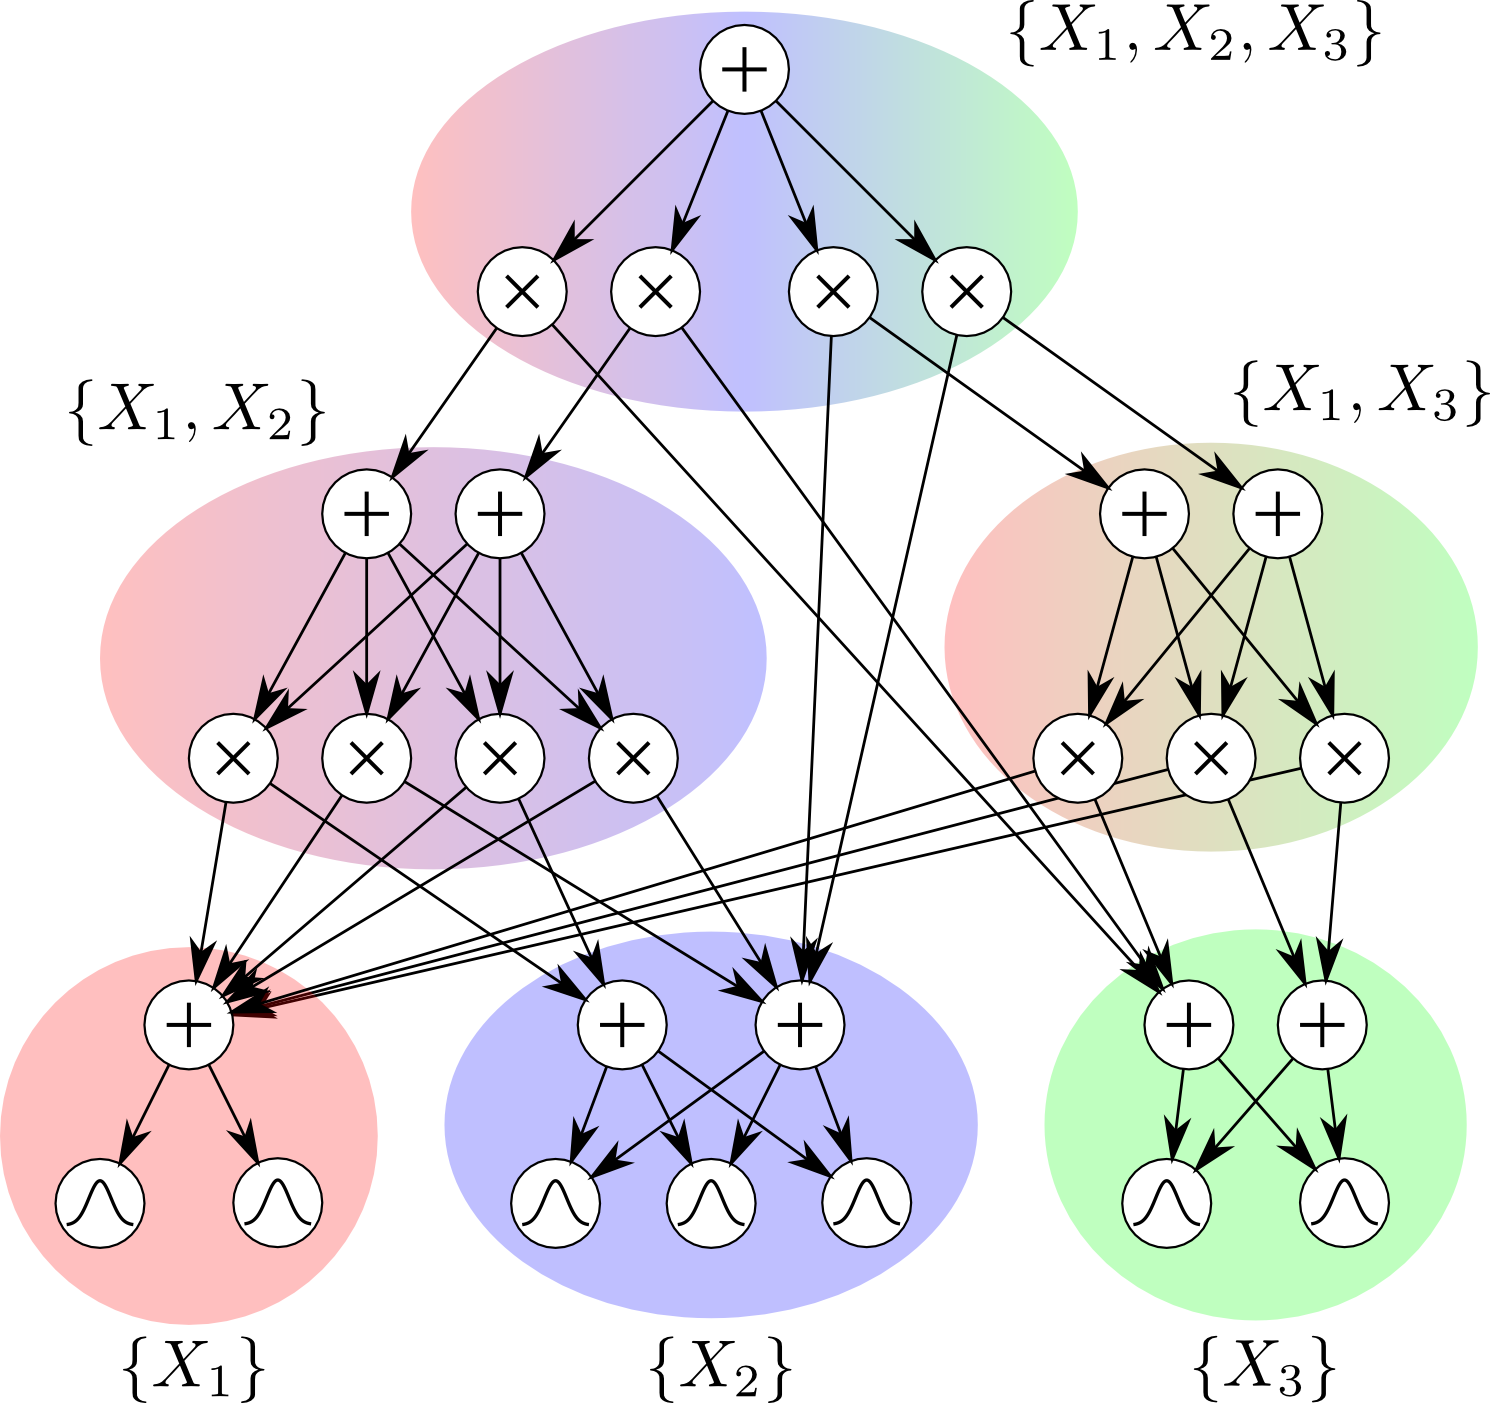
\includegraphics[width=0.4\linewidth]{spn}%
    \hfill
    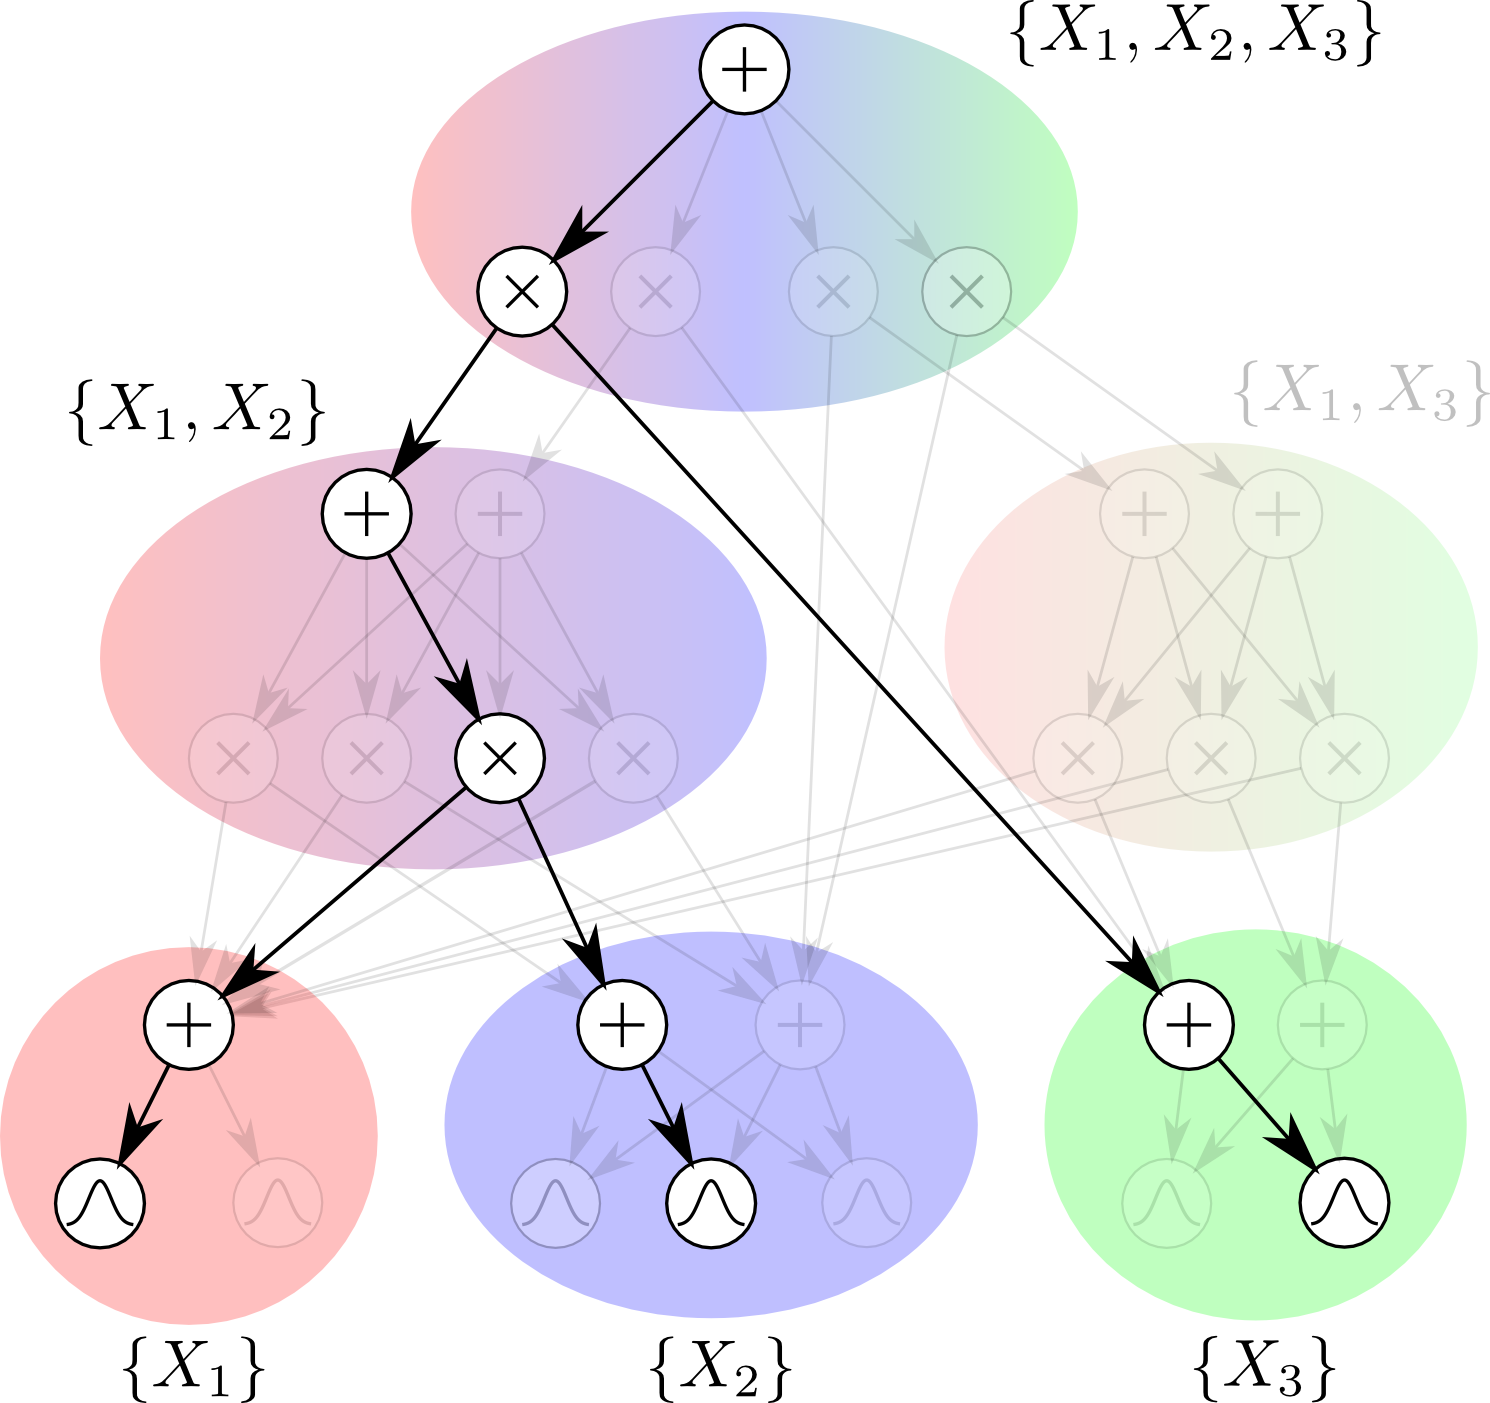
\includegraphics[width=0.4\linewidth]{inducedTree}
    \caption{Illustration of a valid SPN (left) and an induced tree inside the SPN (right). Colored circles indicate the scope of the nodes and are only for illustrative purposes.}%
    \label{fig:inducedTree}%
\end{figure}

\subsection{Gaussian Process} \label{sec:gps}
A Gaussian process (GP) is a distribution over functions which can be applied for classification or regression problems.
In the following discussion we will focus on the use of GPs for regression.
Further we will assume that the prior mean is $0$ and let $\theta = \{\alpha, \sigma_{\epsilon}\}$ denote the parameters of the GP for which $\alpha$ is a kernel specific hyper-parameter and $\sigma_{\epsilon}$ the variance of the noise model assumed, i.e. $\epsilon \sim \N(0, \sigma_{\epsilon}^2)$.
Given a set of training data $\data = \{(\xn, y_n)\}_{n=1}^{N}$ we can optimize the parameters of a GP by minimizing the negative log marginal likelihood, i.e.
\begin{equation}
  \loss = - \log p(\y | \X, \theta) = \frac{1}{2} \log \det(\C) + \frac{1}{2}(\y^T \C^{-1} \y) + \frac{N}{2} \log 2\pi
\end{equation}
where $\C = \K + \sigma^2_{\epsilon}$ and $\K_{ij} = k(\x_i, \x_j)$ being the covariance matrix / kernel matrix and $k(\x_i, \x_j)$ an appropriate covariance function / kernel function.
Given some hyper-parameters and the training data, our main goal is to estimate a prediction for an unseen data point $\x\new$. 
We are therefore interested in the posterior predictive distribution, i.e. $p(\y\new | \x\new, \data)$.
First consider the joint training and testing marginal likelihood for a test samples $\X\new$, which is
\[
  p(\y, \y\new) = \N(\bm 0, \left[\begin{array}{cc}
\K_{N,N} + \sigma^2_{\epsilon}I & \K_{N,\new} \\
\K_{\new,N} & \K_{\new,\new} \end{array} \right]) \, .
\]
For a single data point $\x\new$ we therefore obtain a posterior predictive which is a Gaussian with mean and variance given by:
\begin{align}
  \mu\new &= \kk_{\new}^T (\K_{N,N} + \sigma^2_{\epsilon}\bm I)^{-1} \y \, ,\\
  \sigma\new &= k(\x\new, \x\new) - \kk_{\new}^T(\K_{N,N} + \sigma^2_{\epsilon}\bm I)^{-1} \kk_{\new} + \sigma^2_{\epsilon} \, ,\\
  \y\new | \x\new, \data &\sim \N(\mu\new, \sigma\new)\, , \label{eq:posteriorGP}
\end{align}
where we use $\kk_{\new}$ as a shorthand for the vector between the test point and the training data.
%Note that for multiple test samples, the posterior predictive distribution is multivariate but for practical reasons often only the diagonal is considered.
%For simplicity, we will therefore always refer to Eq.~\ref{eq:posteriorGP} if we talk about the posterior predictive of a GP.

\section{Merging Gaussian Processes with Sum-Product Networks}
In the following section we will discuss a few possibilities to combine SPNs with GPs.
The most natural way to think about utilizing SPNs for learning of GPs is a hierarchical experts model.
We can divide GP experts approaches into Product of Experts (PoE) based approaches or Mixture of Experts (MoE) based approaches. We will briefly review those approaches.
\subsection{Product of Experts}
A PoE based approach, such as those described in \cite{Deisenroth2015}, assumes a factorised marginal likelihood into $M$ independent GPs, i.e.
\[
  p(\y | \X, \theta) \approx \prod_{m=1}^M p_m(\y_m | \X_m, \theta) \, ,
\]
with shared hyper-parameters $\theta$. Note that $\y_m = \{y_n : z_n = m\}$ and $\X_m = \{\xn : z_n = m\}$ where $\bm z = \{z_n\}_{n=1}^N$ are latent assignments of the training samples to the $M$ independent experts.
Such an approach however, results in a predictive posterior distribution which depends on all GPs.
In particular, in the PoE framework the function value of an unseen data point is estimated based on the product of all independent GPs resulting in straight forward computation of the mean and variance, i.e. the product of  Gaussians PDFs is again Gaussian.
The mean and variance are given by:
\begin{align}
  \mu\new &= \sigma\new^2 \sum_{m=1}^M \sigma_m^{-2}(\x\new) \mu_m(\x\new) \, , \\
  \sigma\new^{-2} &= \sum_{m=1}^M \sigma_m^{-2}(\x\new) \, .
\end{align}
which indicates one of the problems arising in PoE models, i.e. with increasing $M$ the predictive variance vanishes and the model is over-confident. 
Moreover, this approach estimates the function value of $\x\new$ based on all independent GPs, even those which are not trained on data which is in the vicinity of $\x\new$.
%The advantage is that such an approach is that it is very easy to realize, as shown in Listing~\ref{lst:poe}, but on the other hand results in 'degenerated' GP.

\subsection{Mixture of Experts}
An alternative approach to the PoE is the use of a mixture or better an infinite mixture such as in \cite{RasmussenG2001}.
This approach leads to a mixture model expression in which the mixture is called a gating network, i.e.
\[
  p(\y | \X, \theta) = \sum_{\bm z} \left[ \prod_{m=1}^M p(\y_m | \X_m, \theta_m) \right] p(\bm z | \X, \alpha) \,
\]
where $\alpha$ are hyper-parameters of the gating network and $\bm z =\{z_n\}_{n=1}^N$ is a configuration indicating the assignments of the data points to experts.
Note that hyper-parameters of the experts under such a model are not shared.
Further note that such an approach marginalizes over possible configurations, which naturally results in a Bayesian nonparametric formulation. 
We can find the assignment of an observation to an expert using Gibbs sampling from the posterior conditional $p(z_n = m | \cdot)$. Given training data points, hyper-parameters and configurations we can estimate the function value of an unseen observation as follows: (1) Estimate the indicator variable $z\new$, (2) estimate the function value solely based on the selected GP:
\begin{align}
  \mu\new &= \sum_{m=1}^M \indic{z\new = m} \mu_m(\x\new) \, , \\
  \sigma\new &= \sum_{m=1}^M \indic{z\new = m} \sigma_m(\x\new) \, .
\end{align}
As a consequence, predictions from this model are based on GPs which have been trained on the region of interest only.
For efficient learning this approach might be problematic as it requires to find an appropriate configuration or average over several configurations of the training data and the indicator $z\new$.
A possible solution for infinite mixtures might be an adaption of the approx. MAP inference approach for DP mixtures by \cite{Raykov2016} which could replace the MCMC step described in \cite{RasmussenG2001}.

\subsection{SPN Mixture of Experts}
We can see that a SPN of GP experts follows directly from the work of \cite{RasmussenG2001} and the fact that we can interpret sum nodes (mixtures) as gating networks.
We can therefore write the resulting model as follows:
\begin{equation} \label{eq:spnGP}
  p(\y | \X, \theta) = \sum_{\z} \left[ \prod_{t=1}^{\tau} \prod_{\Leaf \in \SPT_{t}} p(\y_t | \X_{t,\scope(\Leaf)}, \theta_{\Leaf}) \right] p(\z | \X, \alpha)
\end{equation}
where $\y_t = \{y_n : z_n = t\}$ and $\X_t = \{\x_n : z_n = t\}$.
As we are interested in efficient learning in GPs, we will assume that the structure as well as a configuration $\z$ is drawn from the posterior using an oracle only once, e.g. variational inference, MAP or any other approximation which does not require sampling.
Therefore, we do not marginalize over the possible configurations anymore and learn the parameters of the GPs by minimize the negative log marginal likelihood for each GP expert at the leaves independently.
We get the conditional:
\[
  p(\y | \X, \z, \theta) = \prod_{t=1}^{\tau} \prod_{\Leaf \in \SPT_{t}} p(\y_t | \X_{t,\scope(\Leaf)}, \theta_{\Leaf})
\]
which can be efficiently optimized and evaluated.
However, this conditional of course does not reflect our uncertainty in $\z$ anymore.
This raises the following issues, (1) we might get a boundary bias, (2) we allow predictions only from a single GP trained over a potentially very small sub-set of training data which might lead to incorrect predictions.
A natural way of dealing with this issues would be to use MCMC instead and compute an expectation over posterior samples.
As SPNs can represent an exponentially large mixture, we can utilize this by recursively defining Eq.~\ref{eq:spnGP} using additional sum nodes in the network.
The resulting model is
\[
  p(\y | \X, \theta) \approx \sum_{k=1}^K w_k p(\y | \X, \z_k, \theta)
\]
where $K$ is exponentially large, due to the recursive structure of SPNs. Observations under such an model are drawn according to a mixture of Gaussians.
However, drawing samples from this posterior predictive distribution is difficult, i.e. in a common scheme we would draw a component according to the mixing proportions which will again lead to selecting a product of independent GPs learned over a small set of training data only. 
One possible solution to this would be to approximate the predictive posterior by a Gaussian distribution, i.e. compute the mixture mean and variance as follows: 
\begin{align}
  \mu(y\new) &= \sum_{k=1}^K w_k \mu_k(\x\new) \, , \\
  \sigma(\x\new) &= \sum_{k=1}^M w_k \sigma^2_k(\x\new) + \sum_{k=1}^K w_k (\mu_k(\x\new))^2 - \left(\sum_{k=1}^K w_k \mu_k(\x\new)\right)^2\ ,
\end{align}
which follows immediately from the fact that the i\ths moment is computed according to:
\[
  \E_{p}[\x^i] = \sum_{k=1}^K w_k \E_{p_k}[x^i] \, .
\]
In general approximating a mixture model, which can assumed to be multi-modal, with a single Gaussian is doubtful.
However, in this case we can justify the approximation by assuming that this mixture computes an estimate of the expectation of an infinite SPN of GP experts.

%\appendix
%\section{Code Examples using GPFlow}
%\lstset{language=Python}
%\lstset{frame=lines}
%\lstset{caption={Code example for PoE model with GPFlow}}
%\lstset{label={lst:poe}}
%\lstset{basicstyle=\footnotesize}
%\begin{lstlisting}
%import gpflow
%
%X, y = ...# read some data
%
%M = 20 # Number of experts
%poe = [] # List of experts
%
%# Generate random splits (we assume that 0 < x < 1)
%splitsPos = np.sort(np.random.rand(experts-1))
%
%# Training of experts
%for (startPos, endPos) in zip(np.hstack([0, splitsPos]), np.hstack([splitsPos, 1])):
%  X_ = X[(X > endPos) & (X >= startPos)]
%  Y_ = Y[(X > endPos) & (X >= startPos)]
%
%
%  k = gpflow.kernels.RBF(1) # Sepecify kernel of choice
%  m = gpflow.models.GPR(np.matrix(X_).T, np.matrix(Y_).T, kern=k)
%  m.compile()
%  m.optimize()
%  poe.append(m)
%    
%# Prediction using PoE
%x = ... # unseen data point    
%    
%ymean = np.zeros(len(M))
%yvar = np.zeros(len(M))
%
%for (mi, m) in enumerate(M):
%  mean, var = m.predict_y(x)
%  ymean[:,mi] = mean[:,0]
%  yvar[:,mi] = var[:,0]
%            
%var =  1 / np.sum(1 / yvar, 1)
%mean = var * np.sum(np.divide(ymean, yvar), 1)
%\end{lstlisting}

\printbibliography

\end{document}


